\begin{figure}[!htb]
  \centering
  \tikzsetnextfilenamesafe{Chapter5/SFC/schematics}
  \begin{tikzpicture}
    \node[inner sep=0] (mesh) at (0,0) {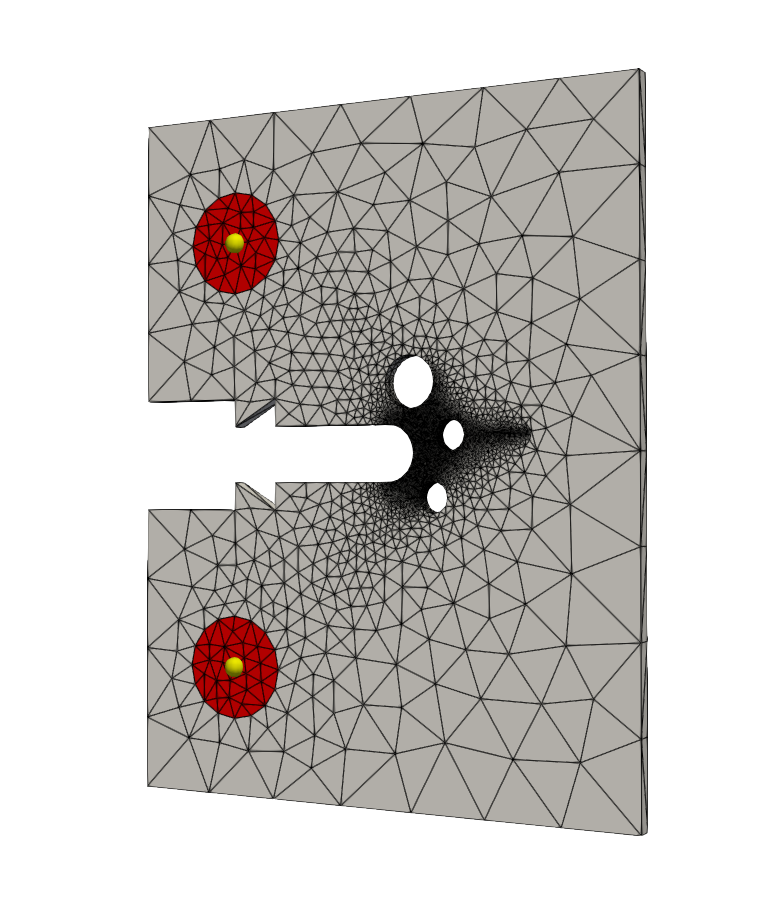
\includegraphics[width=0.3\textwidth,scale=0.5]{Chapter5/figures/SFC/mesh}};
    \coordinate (box_sw) at (-0.2, -0.6);
    \coordinate (box_nw) at (-0.2, 0.78);
    \coordinate (box_ne) at (1, 0.9);
    \coordinate (box_se) at (1, -0.65);
    
    \draw [blue] (box_sw) -- (box_nw);
    \draw [blue] (box_nw) -- (box_ne);
    \draw [blue] (box_ne) -- (box_se);
    \draw [blue] (box_se) -- (box_sw);
    
    \node[inner sep=0] (meshzoom) at (7,0) {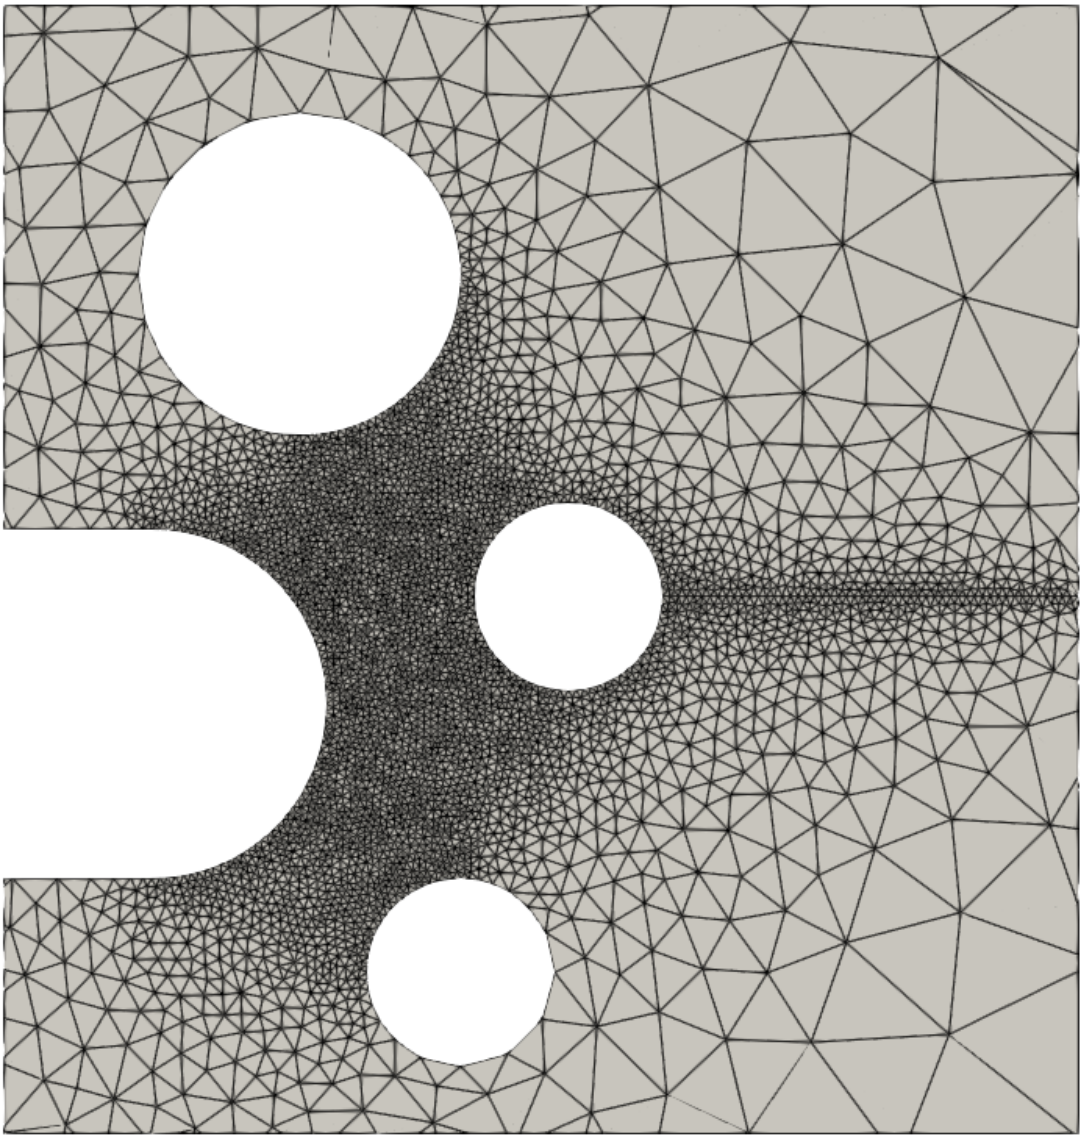
\includegraphics[width=0.3\textwidth,scale=0.5]{Chapter5/figures/SFC/meshzoom}};
    \node (boxzoom) at (meshzoom.south west) [draw,blue,thick,minimum width=0.3\textwidth,minimum height=147,anchor=south west] {};
    
    \draw (box_ne) -- (boxzoom.north west);
    \draw (box_se) -- (boxzoom.south west);
    
    \node (A) at (-1.2,1.6) [yellow] {\textbf{A}};
    \node (B) at (-1.2,-1.7) [yellow] {\textbf{B}};
  \end{tikzpicture}
  \caption{Sandia Fracture Challenge problem geometry and mesh, with zoomed-in view of the refined region. The specimen is loaded vertically with displacement control at lines of nodes A and B marked as yellow spheres.}
  \label{fig: Chapter5/SFC/schematics}
\end{figure}
